% ClimaSense architecture diagram
% Compile on Overleaf (free) or with: pdflatex architecture.tex
\documentclass[border=8pt]{standalone}
\usepackage{tikz}
\usetikzlibrary{positioning, shapes.geometric, arrows.meta, fit, backgrounds, calc}

\begin{document}
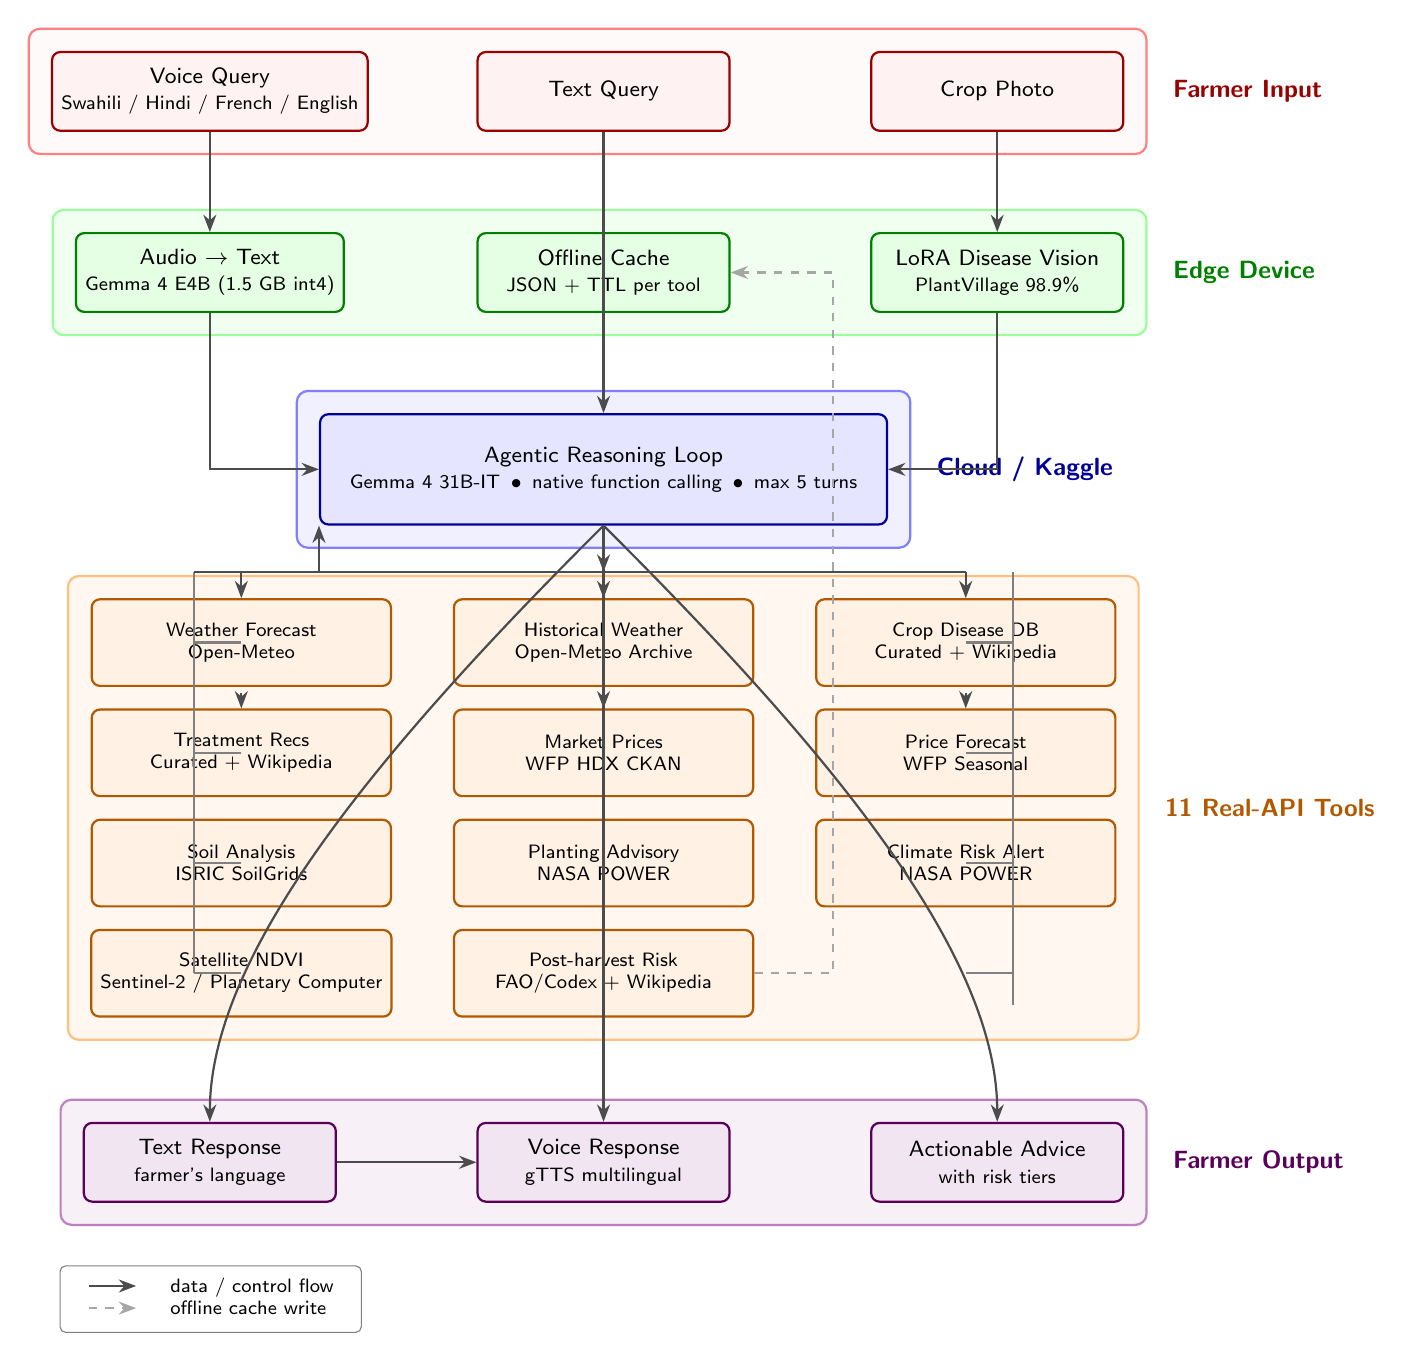
\begin{tikzpicture}[
    font=\sffamily\small,
    >={Stealth[length=2.2mm]},
    layer/.style={rounded corners=4pt, thick, inner sep=8pt},
    box/.style={
        rectangle, rounded corners=3pt, draw, thick,
        minimum width=32mm, minimum height=10mm,
        align=center, fill=white, font=\sffamily\footnotesize
    },
    tool/.style={
        box, minimum width=38mm, minimum height=11mm,
        font=\sffamily\scriptsize
    },
    inputbox/.style={box, fill=pink!20, draw=red!60!black},
    edgebox/.style={box, fill=green!10, draw=green!50!black},
    cloudbox/.style={box, fill=blue!10, draw=blue!60!black, minimum width=72mm, minimum height=14mm},
    toolbox/.style={tool, fill=orange!10, draw=orange!70!black},
    outputbox/.style={box, fill=violet!10, draw=violet!70!black},
    flow/.style={->, thick, draw=black!70},
    cacheflow/.style={->, thick, dashed, draw=gray!70},
]

% =====================================================================
% Row Y-coordinates (top to bottom). Spaced to avoid any overlap.
% =====================================================================
% y =  0   Input row
% y = -2.0 Edge row
% y = -4.5 Cloud row (agent)
% y = -7.5 Tools grid (4 rows of 3 = -7.0, -8.2, -9.4, -10.6)
% y = -12.5 Output row

% ---------- INPUT LAYER ----------
\node[inputbox] (voice) at (-5, 0)  {Voice Query\\\scriptsize Swahili / Hindi / French / English};
\node[inputbox] (text)  at ( 0, 0)  {Text Query};
\node[inputbox] (photo) at ( 5, 0)  {Crop Photo};

% ---------- EDGE LAYER ----------
\node[edgebox] (transcribe) at (-5, -2.3) {Audio $\rightarrow$ Text\\\scriptsize Gemma 4 E4B (1.5 GB int4)};
\node[edgebox] (cache)      at ( 0, -2.3) {Offline Cache\\\scriptsize JSON + TTL per tool};
\node[edgebox] (lora)       at ( 5, -2.3) {LoRA Disease Vision\\\scriptsize PlantVillage 98.9\%};

% ---------- CLOUD LAYER ----------
\node[cloudbox] (agent) at (0, -4.8) {
    Agentic Reasoning Loop \\
    \scriptsize Gemma 4 31B-IT \,$\bullet$\, native function calling \,$\bullet$\, max 5 turns
};

% ---------- TOOLS GRID (3 columns x 4 rows) ----------
\def\tx{4.6}                          % column spacing
\def\tyA{-7.0}\def\tyB{-8.4}
\def\tyC{-9.8}\def\tyD{-11.2}

\node[toolbox] (t1)  at (-\tx, \tyA) {Weather Forecast\\\scriptsize Open-Meteo};
\node[toolbox] (t2)  at (   0, \tyA) {Historical Weather\\\scriptsize Open-Meteo Archive};
\node[toolbox] (t3)  at ( \tx, \tyA) {Crop Disease DB\\\scriptsize Curated + Wikipedia};

\node[toolbox] (t4)  at (-\tx, \tyB) {Treatment Recs\\\scriptsize Curated + Wikipedia};
\node[toolbox] (t5)  at (   0, \tyB) {Market Prices\\\scriptsize WFP HDX CKAN};
\node[toolbox] (t6)  at ( \tx, \tyB) {Price Forecast\\\scriptsize WFP Seasonal};

\node[toolbox] (t7)  at (-\tx, \tyC) {Soil Analysis\\\scriptsize ISRIC SoilGrids};
\node[toolbox] (t8)  at (   0, \tyC) {Planting Advisory\\\scriptsize NASA POWER};
\node[toolbox] (t9)  at ( \tx, \tyC) {Climate Risk Alert\\\scriptsize NASA POWER};

\node[toolbox] (t10) at (-\tx, \tyD) {Satellite NDVI\\\scriptsize Sentinel-2 / Planetary Computer};
\node[toolbox] (t11) at (   0, \tyD) {Post-harvest Risk\\\scriptsize FAO/Codex + Wikipedia};

% ---------- OUTPUT LAYER ----------
\node[outputbox] (otext)  at (-5, -13.6) {Text Response\\\scriptsize farmer's language};
\node[outputbox] (ovoice) at ( 0, -13.6) {Voice Response\\\scriptsize gTTS multilingual};
\node[outputbox] (oadv)   at ( 5, -13.6) {Actionable Advice\\\scriptsize with risk tiers};

% ---------- LAYER BACKGROUNDS ----------
\begin{scope}[on background layer]
    \node[layer, fill=pink!8, draw=red!50, fit=(voice)(photo)] (inputlayer) {};
    \node[layer, fill=green!6, draw=green!40, fit=(transcribe)(lora)] (edgelayer) {};
    \node[layer, fill=blue!6,  draw=blue!50,  fit=(agent)] (cloudlayer) {};
    \node[layer, fill=orange!6, draw=orange!50,
          fit=(t1)(t3)(t10)(t11)] (toollayer) {};
    \node[layer, fill=violet!6, draw=violet!50, fit=(otext)(oadv)] (outputlayer) {};
\end{scope}

% ---------- LAYER LABELS (right side, no overlap) ----------
\node[anchor=west, font=\sffamily\bfseries\small, text=red!60!black]
    at ($(inputlayer.east) + (0.2, 0)$) {Farmer Input};
\node[anchor=west, font=\sffamily\bfseries\small, text=green!50!black]
    at ($(edgelayer.east)  + (0.2, 0)$) {Edge Device};
\node[anchor=west, font=\sffamily\bfseries\small, text=blue!60!black]
    at ($(cloudlayer.east) + (0.2, 0)$) {Cloud / Kaggle};
\node[anchor=west, font=\sffamily\bfseries\small, text=orange!70!black]
    at ($(toollayer.east)  + (0.2, 0)$) {11 Real-API Tools};
\node[anchor=west, font=\sffamily\bfseries\small, text=violet!70!black]
    at ($(outputlayer.east)+ (0.2, 0)$) {Farmer Output};

% ---------- INPUT -> EDGE / CLOUD ----------
\draw[flow] (voice) -- (transcribe);
\draw[flow] (text.south)  -- ++(0,-0.4) -| (agent.north);
\draw[flow] (photo) -- (lora);
\draw[flow] (transcribe.south) |- ($(agent.west) + (-0.3, 0)$) -- (agent.west);
\draw[flow] (lora.south)       |- ($(agent.east) + ( 0.3, 0)$) -- (agent.east);

% ---------- AGENT -> TOOLS (single fan-out via bus) ----------
\coordinate (busTop) at (0, -6.1);
\coordinate (busLeft)  at (-\tx, -6.1);
\coordinate (busRight) at ( \tx, -6.1);
\draw[flow] (agent.south) -- (busTop);
\draw[thick, draw=black!70] (busLeft) -- (busRight);
\foreach \t in {t1, t2, t3} { \draw[flow] (busLeft -| \t.north) -- (\t.north); }

% Inter-row connectors (right side) so rows 2-4 receive flow without crossing
\foreach \t in {t4, t5, t6} { \draw[flow] (\t.north) ++(0,0.2) -- (\t.north); }
\draw[thick, draw=black!50] (busRight) ++(0.6,0) -- ++(0,-5.5)
    coordinate (sideBus);
\foreach \y in {\tyA, \tyB, \tyC, \tyD} {
    \draw[thick, draw=black!50] (\tx + 0.6, \y) -- (\tx + 0.0, \y);
}

% Tool results flow back to agent (left-side return bus)
\draw[thick, draw=black!50] (-\tx - 0.6, -6.1) -- (-\tx - 0.6, \tyD);
\foreach \y in {\tyA, \tyB, \tyC, \tyD} {
    \draw[thick, draw=black!50] (-\tx, \y) -- (-\tx - 0.6, \y);
}
\draw[flow] (-\tx - 0.6, -6.1) -| (agent.south west);

% ---------- TOOLS -> CACHE (dashed, persistence) ----------
\draw[cacheflow] (t11.east) -- ++(1.0, 0) |- (cache.east);

% ---------- AGENT -> OUTPUTS ----------
\draw[flow] (agent.south) ++(0,-0.0) .. controls (-3, -8.5) and (-5, -11) .. (otext.north);
\draw[flow] (agent.south) -- ++(0,-0.4) -| (ovoice.north);
\draw[flow] (agent.south) ++(0,-0.0) .. controls ( 3, -8.5) and ( 5, -11) .. (oadv.north);
\draw[flow] (otext) -- (ovoice);

% ---------- LEGEND ----------
\node[anchor=north west, font=\sffamily\scriptsize, draw=black!50, rounded corners=2pt,
      inner sep=4pt, fill=white]
    at ($(outputlayer.south west) + (0, -0.5)$) {
    \begin{tabular}{ll}
        \tikz\draw[flow] (0,0)--(0.6,0); & data / control flow \\
        \tikz\draw[cacheflow] (0,0)--(0.6,0); & offline cache write \\
    \end{tabular}
};

\end{tikzpicture}
\end{document}
